\begin{longtable} { | c | p{12cm} | c | } 
\hline
	ID 	&	Issues	&		 Es. hours \\\hline
	38	&	Create nested sequence placeholder	&	2 hours \\\hline
	39 	&	Create choice placeholder	&	2 hours \\\hline
\caption{Issue ID 39}
\label{tab:spr3_choiceplaceholder}
\end{longtable}

With the addition of nested and choice functionality to sequences, we needed a way to easily identify these elements within a sequence. Initially, a frame consisting of a choice would be displayed using the first pictogram of that choice. A frame consisting of a nested sequence would have the first pictogram in that sequence. Without remembering what the frames were, it was impossible to distinguish these special frames from other pictograms in the sequence without clicking on them. This would result in different behavior, depending on what was clicked. To solve this issue, hardcoded placeholders were temporarily created, replacing all pictograms with placeholders. These would identify them as pictograms, choices or nested sequences. The following figures are the placeholders used in Sekvens.

\begin{figure} [h!]
\centering
\begin{minipage}{.3\textwidth}
\centering
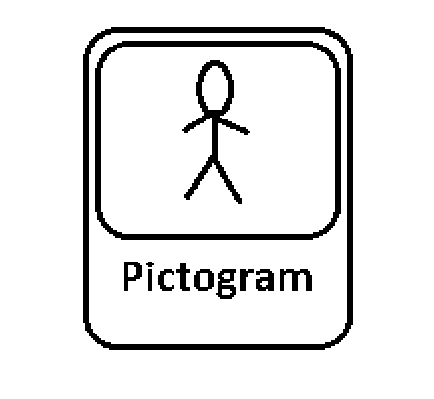
\includegraphics[scale=0.5]{Pics/Sprint3/placeholders/PLACEHOLDER_PICTOGRAM.png}
\caption{The placeholder for a pictogram}
\label{fig:placePictogram}
\end{minipage}\hfill
\begin{minipage}{.3\textwidth}
\centering
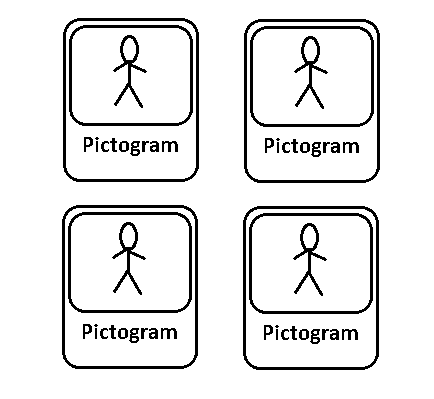
\includegraphics[scale=0.5]{Pics/Sprint3/placeholders/PLACEHOLDER_SEQUENCE.png}
\caption{The placeholder for a sequence}
\label{fig:placeSequence}
\end{minipage}\hfill
\begin{minipage}{.3\textwidth}
\centering
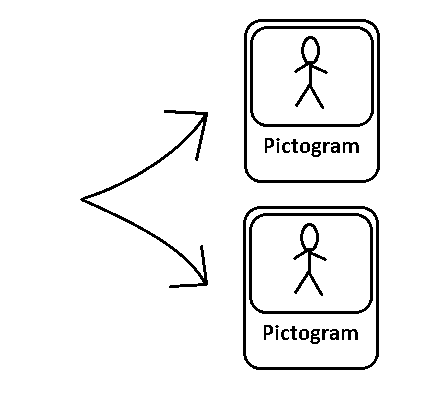
\includegraphics[scale=0.5]{Pics/Sprint3/placeholders/PLACEHOLDER_VALG.png}
\caption{The placeholder for a placeholder}
\label{fig:placeChoice}
\end{minipage}
\end{figure}